\subsection{Stability under changes of the Mapper parameters}
\label{sec:stability}

We varied the lens (PCA, distance to the centroid), the number of intervals
(10, 15, 20) and the overlap (0.3, 0.5, 0.7), keeping average linkage at 0.27,
and ran the Mapper selector on the same 30 ingestions (3 trap types, 10 seeds,
20 chunks each). Each setting is compared with the default (PCA, 15 intervals,
0.5) on the same ingestion. Figure~\ref{fig:stability} shows the budget of 30
questions (10\%); Table~\ref{tab:stability} has all three budgets.
\texttt{python experiments/stability.py} reproduces both.

The stability theorem of \cite{carriere2018structure} does not apply here: it
needs a lens of Morse type and a gomic, and our cover with overlap $0.5$ is not
a gomic and is clustered with average linkage on a point cloud
(\S\ref{sec:mapper}). The results below are therefore empirical.

\paragraph{What the selection finds is stable.} The 30 ingestions break only
14 questions, in 11 of them, so one question moves the detection rate by 7
points. We therefore also count the 600 target questions, the ones the traps
were written against. At the 10\% budget every setting selects between 34\%
and 47\% of the targets (default 39\%), against 10\% for a random selection of
the same size; at 20\% it selects 64--79\% (default 70\%, random 20\%). The
detection rate at 20\% ranges from 57\% to 93\% (default 79\%), that is, between
8 and 13 of the 14 broken questions. At 10\% it spreads more, from 14\% to 71\%:
2 to 10 questions, within the noise that 14 questions allow.

\paragraph{Which questions it selects is less stable.} The overlap sets the
size of the marked region: with overlap 0.3 between 112 and 185 of the 300
questions are candidates, with 0.7 between 253 and 268. The candidate sets
share 49--71\% of their questions with the default's (Jaccard). The 30 selected
questions share less: Jaccard 0.36--0.49 for the PCA lens and 0.29--0.35 for the
centroid lens, against about 0.09 for two random selections of 30 among 190
candidates. The centroid lens marks regions as close to the default as PCA
does, but orders them differently. Inside a region, many questions tie on the
two ranking keys (affected tier, new chunks in the node) and the tie goes to the
question id, so a small change of the region changes which tied questions fit
in the budget.

\paragraph{Reading.} Changing the cover moves the boundaries of the marked
region and reorders the questions inside it, but every setting still puts the
targets of the ingestion near the top, three to four times more often than
chance. The method is stable in how much it finds and not in which questions it
lists, so a single list should not be read as \emph{the} set of affected
questions. A ranking key that breaks the ties by geometry, such as the
similarity to the nearest new chunk, is the obvious next step. These numbers
come from one corpus, one ingestion size and rare breaks; the detection rates
in particular rest on 14 questions.

\begin{figure}[htbp]
  \centering
  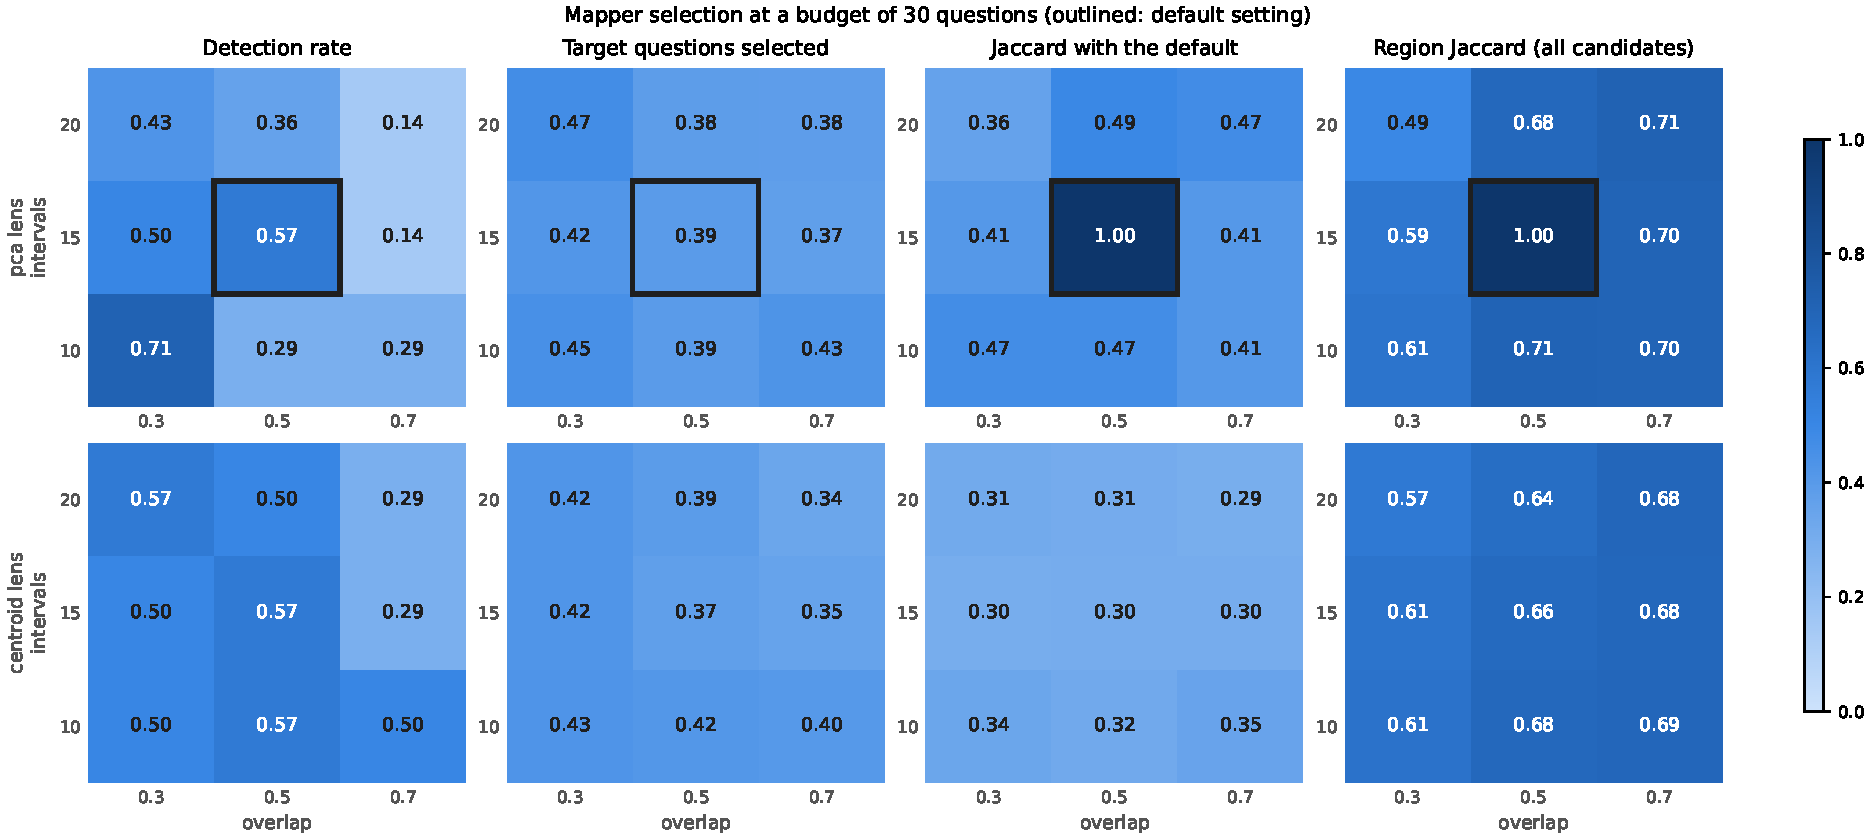
\includegraphics[width=\textwidth]{figures/stability_heatmap.pdf}
  \caption{Mapper selection at a budget of 30 of 300 questions, pooled over 30
  ingestions, for each lens, number of intervals and overlap. Detection rate:
  broken questions selected. Target questions selected: questions the traps
  were written against. Jaccard with the default: overlap of the 30 selected
  questions with those of the default setting (outlined). Region Jaccard: the
  same for the whole candidate sets.}
  \label{fig:stability}
\end{figure}

\begin{table}[htbp]
  \centering
  \scriptsize
  % Generated by experiments/stability.py; do not edit by hand.
\begin{tabular}{lrrrrrrrrrrrrr}
\hline
 & & & & & \multicolumn{3}{c}{budget 15} & \multicolumn{3}{c}{budget 30} & \multicolumn{3}{c}{budget 60} \\
Lens & Int. & Ov. & Cand. & Region & Det. & Targ. & Jacc. & Det. & Targ. & Jacc. & Det. & Targ. & Jacc. \\
\hline
pca & 10 & 0.3 & 160 & 0.61 & 14\% & 25\% & 0.39 & 71\% & 45\% & 0.47 & 86\% & 77\% & 0.50 \\
pca & 10 & 0.5 & 214 & 0.71 & 14\% & 21\% & 0.39 & 29\% & 39\% & 0.47 & 86\% & 71\% & 0.50 \\
pca & 10 & 0.7 & 256 & 0.70 & 14\% & 22\% & 0.34 & 29\% & 43\% & 0.41 & 86\% & 78\% & 0.47 \\
pca & 15 & 0.3 & 145 & 0.59 & 7\% & 22\% & 0.34 & 50\% & 42\% & 0.41 & 71\% & 73\% & 0.48 \\
\textbf{pca} & 15 & 0.5 & 190 & 1.00 & 14\% & 20\% & 1.00 & 57\% & 39\% & 1.00 & 79\% & 70\% & 1.00 \\
pca & 15 & 0.7 & 257 & 0.70 & 14\% & 18\% & 0.35 & 14\% & 37\% & 0.41 & 79\% & 69\% & 0.49 \\
pca & 20 & 0.3 & 112 & 0.49 & 29\% & 27\% & 0.31 & 43\% & 46\% & 0.36 & 57\% & 76\% & 0.43 \\
pca & 20 & 0.5 & 175 & 0.68 & 0\% & 21\% & 0.42 & 36\% & 38\% & 0.49 & 64\% & 71\% & 0.52 \\
pca & 20 & 0.7 & 253 & 0.71 & 14\% & 20\% & 0.40 & 14\% & 38\% & 0.47 & 71\% & 68\% & 0.52 \\
centroid & 10 & 0.3 & 185 & 0.61 & 14\% & 20\% & 0.24 & 50\% & 43\% & 0.34 & 86\% & 79\% & 0.40 \\
centroid & 10 & 0.5 & 232 & 0.68 & 14\% & 21\% & 0.23 & 57\% & 42\% & 0.32 & 86\% & 76\% & 0.42 \\
centroid & 10 & 0.7 & 263 & 0.69 & 29\% & 20\% & 0.29 & 50\% & 40\% & 0.35 & 93\% & 75\% & 0.44 \\
centroid & 15 & 0.3 & 168 & 0.61 & 14\% & 22\% & 0.20 & 50\% & 42\% & 0.30 & 57\% & 75\% & 0.39 \\
centroid & 15 & 0.5 & 216 & 0.66 & 29\% & 18\% & 0.19 & 57\% & 37\% & 0.30 & 93\% & 68\% & 0.39 \\
centroid & 15 & 0.7 & 266 & 0.68 & 21\% & 17\% & 0.24 & 29\% & 35\% & 0.30 & 64\% & 64\% & 0.40 \\
centroid & 20 & 0.3 & 156 & 0.57 & 43\% & 21\% & 0.23 & 57\% & 42\% & 0.31 & 71\% & 72\% & 0.37 \\
centroid & 20 & 0.5 & 190 & 0.64 & 21\% & 20\% & 0.20 & 50\% & 39\% & 0.31 & 86\% & 72\% & 0.40 \\
centroid & 20 & 0.7 & 268 & 0.68 & 29\% & 17\% & 0.20 & 29\% & 34\% & 0.29 & 64\% & 64\% & 0.41 \\
\hline
\end{tabular}

  \caption{Stability of the Mapper selection. Cand.: mean number of candidate
  questions. Region: Jaccard of the candidate set with the default's. For each
  budget: detection rate, target questions selected, and Jaccard of the selection
  with the default's. The default setting is in bold.}
  \label{tab:stability}
\end{table}
